%
% j1a SwapForth manual
%

\input{../../doc/front.tex}

\title{\LARGE \bf
J1a\\
SwapForth \\
Reference
}

\begin{document}

\maketitle

%% copyrightpage
\begingroup
\footnotesize
\parindent 0pt
\parskip \baselineskip
\textcopyright{} 2015, James Bowman \\
All rights reserved \\
Adapted to Olimex ICE40 board by pbrier (pbrier@pbrier.nl)
\begin{framed}

\underline{ANS Forth Compliance Label}

J1a SwapForth is an ANS Forth System

Providing names from the \wl{Core Extensions} word set \\
Providing names from the \wl{Double-Number} word set \\
% Providing the \wl{Double-Number Extensions} word set \\
% Providing the \wl{Exception} word set \\
Providing names from the \wl{Facility} word set \\
Providing names from the \wl{Facility Extensions} word set \\
% Providing names from the \wl{File Access} word set \\
% Providing names from the \wl{File Access Extensions} word set \\
% Providing names from the \wl{Floating-Point} word set \\
% Providing names from the \wl{Floating-Point Extensions} word set \\
% Providing the \wl{Memory-Allocation} word set \\
% Providing the \wl{Search-Order} word set \\
% Providing the \wl{Search-Order Extensions} word set \\
Providing names from the \wl{String} word set \\
Providing names from the \wl{Programming-Tools} word set \\
Providing names from the \wl{Programming-Tools Extensions} word set

\end{framed}

\endgroup

\thispagestyle{empty}
\pagestyle{headings}

\tableofcontents

%%%%%%%%%%%%%%%%%%%%%%%%%%%%%%%%%%%%%%%%%%%%%%%%%%%%%%%%%%%%%%%%%%%%%%%%
\chapter{Getting started}

\begin{center}
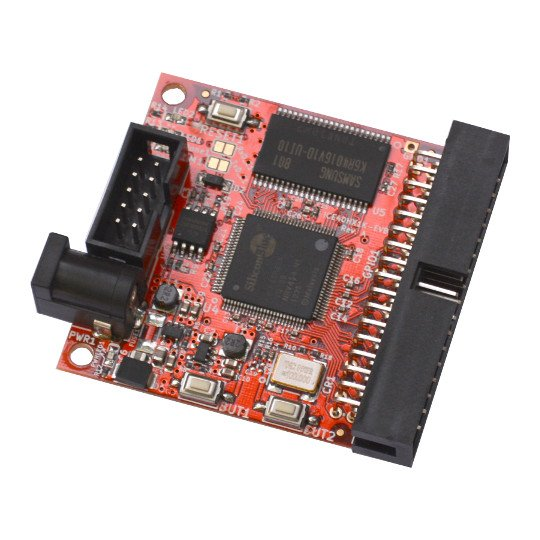
\includegraphics[width=0.6\textwidth]{iCE40HX1K-EVB-1.jpg}
\end{center}

J1a SwapForth is a 16-bit version of SwapForth,
intended as an interactive Forth system using very little logic and RAM.
The system currently fits on a Lattice iCE40HX-1k FPGA. \index{FPGA}
The J1a and peripherals use 1200 logic elements.
SwapForth uses 4.7 Kbytes of RAM,
leaving about 3.3 Kbytes for the application. \index{RAM}. This version is adapted to run on an \href{https://www.olimex.com/Products/FPGA/iCE40/iCE40HX1K-EVB/open-source-hardware}{Olimex ICE40 board} and is compiled using the all open source \href{http://www.clifford.at/icestorm/}{icestorm} toolchain. Access to the on-board LEDs (2x), BUTTONs (2x), SRAM (512kbyte), SPI FLASH (2MByte) and GPIO (16-bit) is implemented. The clock frequency is 50MHz.   

\newpage
After installing the \href{http://www.clifford.at/icestorm/}{icestorm}, \href{https://gist.github.com/derhuerst/1b15ff4652a867391f03}{git}, and the \href{https://www.olimex.com/wiki/ICE40HX1K-EVB#Get_started_under_Linux}{Olimex Arduino or RPi programmer tools} you can install and run it on an
\href{https://www.olimex.com/Products/FPGA/iCE40/iCE40HX1K-EVB/open-source-hardware}{Olimex ICE40 board} 
like this

\begin{framed}
\begin{Verbatim}
  git clone https://github.com/pbrier/swapforth.git
  cd swapforth/j1a
  iceprogduino olimex-ice40/j1a.bin
  python shell.py -h /dev/ttyUSB0
\end{Verbatim}
\end{framed}

\noindent
(where \mach{/dev/ttyUSB0} is the appropriate port your serial adaptor was assigned).
You should see something like

\begin{framed}
\begin{Verbatim}
  Contacting... established
  Loaded 208 words
  >
\end{Verbatim}
\end{framed}

And you can now try the usual Forth things, e.g.

\begin{framed}
\begin{Verbatim}[commandchars=\\\{\}]
\underline{\textbf{1 2 + .}}
3   ok
\end{Verbatim}
\end{framed}

There is a fairly complete 
\href{http://forth.sourceforge.net/std/dpans/dpans6.htm}{core ANS-compatible Forth system}
running on the board, including a compiler.

\newpage
\section{Some demos} \index{demos}

You can control the two on-board LEDs \index{LEDs}

\begin{framed}
\begin{Verbatim}[commandchars=\\\{\}]
\underline{\textbf{-1 leds}}
  ok

\underline{\textbf{0 leds}}
  ok
\end{Verbatim}
\end{framed}

\noindent
and to make them blink

\begin{framed}
\begin{Verbatim}[commandchars=\\\{\}]
: blink
  32 0 do
    i leds
    100 ms
  loop
;
blink
\end{Verbatim}
\end{framed}

\input{../../doc/easter.tex}

\newpage
\section{Building from scratch}

After installing the icestorm tools, run

\begin{Verbatim}
~/Documents/ice/swapforth/j1a $ make clean
~/Documents/ice/swapforth/j1a $ make j1a
\end{Verbatim}

\noindent
This will produce \mach{j1a.bin} - but it only contains the very bare-bones system;
the rest of SwapForth still needs to be compiled.
To do this, load \mach{j1a.bin} and start the shell
(assuming your board's serial appears at \mach{ttyUSB0}):

\begin{framed}
\begin{Verbatim}
  $ iceprogduino olimex-ice40/j1a.bin
  $ python shell.py -h /dev/ttyUSB0 -p ../common/
  Contacting... established
  Loaded 143 words
  _
\end{Verbatim}
\end{framed}

Then compile the rest of SwapForth and write the finished executable with these commands:

\begin{framed}
\begin{Verbatim}
  #include swapforth.fs
  #flash build/nuc.hex
  #bye
\end{Verbatim}
\end{framed}

Now run \mach{make -C olimex-ice40} again - this compiles an FPGA image with the complete code base built-in,
which has the full set of words defined:

\begin{framed}
\begin{Verbatim}
  $ iceprogduino olimex-ice40/j1a.bin
  $ python shell.py -h /dev/ttyUSB0 -p ../common/
  Contacting... established
  Loaded 207 words
\end{Verbatim}
\end{framed}

%%%%%%%%%%%%%%%%%%%%%%%%%%%%%%%%%%%%%%%%%%%%%%%%%%%%%%%%%%%%%%%%%%%%%%%%

\chapter{Available Words}

\section{ANS Core Words} \index{ANS}

J1a SwapForth implements most of the core ANS 94 Forth standard.
Implemented words are:

\input{../../doc/core.tex}

\noindent
The core word
\word{environment?}
is not implemented.
J1a SwapForth also implements the following standard words:

\href{http://forth.sourceforge.net/std/dpans/dpans6.htm#6.2.0200}{\wordidx{.(}}
\href{http://forth.sourceforge.net/std/dpans/dpans6.htm#6.2.0210}{\wordidx{.r}}
\href{http://forth.sourceforge.net/std/dpans/dpans15.htm#15.6.1.0220}{\wordidx{.s}}
\href{http://forth.sourceforge.net/std/dpans/dpans17.htm#17.6.1.0245}{\wordidx{/string}}
\href{http://forth.sourceforge.net/std/dpans/dpans6.htm#6.2.0260}{\wordidx{0<>}}
\href{http://forth.sourceforge.net/std/dpans/dpans6.htm#6.2.0280}{\wordidx{0>}}
\href{http://forth.sourceforge.net/std/dpans/dpans6.htm#6.2.0455}{\wordidx{:noname}}
\href{http://forth.sourceforge.net/std/dpans/dpans6.htm#6.2.0500}{\wordidx{<>}}
\href{http://forth.sourceforge.net/std/dpans/dpans6.htm#6.2.0620}{\wordidx{?do}}
\href{http://forth.sourceforge.net/std/dpans/dpans6.htm#6.2.0700}{\wordidx{again}}
\href{http://forth.sourceforge.net/std/dpans/dpans15.htm#15.6.2.0702}{\wordidx{ahead}}
\href{http://forth.sourceforge.net/std/dpans/dpans6.htm#6.2.0873}{\wordidx{case}}
\href{http://forth.sourceforge.net/std/dpans/dpans17.htm#17.6.1.0910}{\wordidx{cmove}}
\href{http://forth.sourceforge.net/std/dpans/dpans17.htm#17.6.1.0920}{\wordidx{cmove>}}
\href{http://forth.sourceforge.net/std/dpans/dpans6.htm#6.2.0945}{\wordidx{compile,}}
\href{http://forth.sourceforge.net/std/dpans/dpans8.htm#8.6.1.1040}{\wordidx{d+}}
\href{http://forth.sourceforge.net/std/dpans/dpans8.htm#8.6.1.1060}{\wordidx{d.}}
\href{http://forth.sourceforge.net/std/dpans/dpans8.htm#8.6.1.1070}{\wordidx{d.r}}
\href{http://forth.sourceforge.net/std/dpans/dpans8.htm#8.6.1.1080}{\wordidx{d0=}}
\href{http://forth.sourceforge.net/std/dpans/dpans8.htm#8.6.1.1090}{\wordidx{d2*}}
\href{http://forth.sourceforge.net/std/dpans/dpans8.htm#8.6.1.1160}{\wordidx{dabs}}
\href{http://forth.sourceforge.net/std/dpans/dpans8.htm#8.6.1.1230}{\wordidx{dnegate}}
\href{http://forth.sourceforge.net/std/dpans/dpans15.htm#15.6.1.1280}{\wordidx{dump}}
\href{http://forth.sourceforge.net/std/dpans/dpans6.htm#6.2.1342}{\wordidx{endcase}}
\href{http://forth.sourceforge.net/std/dpans/dpans6.htm#6.2.1343}{\wordidx{endof}}
\href{http://forth.sourceforge.net/std/dpans/dpans6.htm#6.2.1350}{\wordidx{erase}}
\href{http://forth.sourceforge.net/std/dpans/dpans6.htm#6.2.1485}{\wordidx{false}}
\href{http://forth.sourceforge.net/std/dpans/dpans6.htm#6.2.1660}{\wordidx{hex}}
\href{http://forth.sourceforge.net/std/dpans/dpans10.htm#10.6.1.1755}{\wordidx{key?}}
\href{http://forth.sourceforge.net/std/dpans/dpans8.htm#8.6.1.1830}{\wordidx{m+}}
\href{http://forth.sourceforge.net/std/dpans/dpans6.htm#6.2.1850}{\wordidx{marker}}
\href{http://forth.sourceforge.net/std/dpans/dpans10.htm#10.6.2.1905}{\wordidx{ms}}
\href{http://forth.sourceforge.net/std/dpans/dpans6.htm#6.2.1930}{\wordidx{nip}}
\href{http://forth.sourceforge.net/std/dpans/dpans6.htm#6.2.1950}{\wordidx{of}}
\href{http://forth.sourceforge.net/std/dpans/dpans6.htm#6.2.2000}{\wordidx{pad}}
\href{http://forth.sourceforge.net/std/dpans/dpans6.htm#6.2.2008}{\wordidx{parse}}
\href{http://forth.sourceforge.net/std/dpans/dpans6.htm#6.2.2125}{\wordidx{refill}}
\href{http://forth.sourceforge.net/std/dpans/dpans6.htm#6.2.2148}{\wordidx{restore-input}}
\href{http://forth.sourceforge.net/std/dpans/dpans6.htm#6.2.2182}{\wordidx{save-input}}
\href{http://forth.sourceforge.net/std/dpans/dpans17.htm#17.6.1.2212}{\wordidx{sliteral}}
\href{http://forth.sourceforge.net/std/dpans/dpans9.htm#9.6.1.2275}{\wordidx{throw}}
\href{http://forth.sourceforge.net/std/dpans/dpans6.htm#6.2.2298}{\wordidx{true}}
\href{http://forth.sourceforge.net/std/dpans/dpans6.htm#6.2.2300}{\wordidx{tuck}}
\href{http://forth.sourceforge.net/std/dpans/dpans6.htm#6.2.2330}{\wordidx{u.r}}
\href{http://forth.sourceforge.net/std/dpans/dpans6.htm#6.2.2350}{\wordidx{u>}}
\href{http://forth.sourceforge.net/std/dpans/dpans6.htm#6.2.2395}{\wordidx{unused}}
\href{http://forth.sourceforge.net/std/dpans/dpans6.htm#6.2.2440}{\wordidx{within}}
\href{http://forth.sourceforge.net/std/dpans/dpans15.htm#15.6.1.2465}{\wordidx{words}}
\href{http://forth.sourceforge.net/std/dpans/dpans6.htm#6.2.2530}{\wordidx{[compile]}}
\href{http://forth.sourceforge.net/std/dpans/dpans6.htm#6.2.2535}{\wordidx{\textbackslash}}

\noindent
Double numbers are supported using the standard \mach{.} suffix.
The Forth 200x number prefixes are supported: \index{Forth 200x}
\mach{\$} for hex,
\mach{\#} for decimal,
\mach{\%} for binary, and \mach{'c'} for character literals.
\href{http://www.forth200x.org/parse-name.html}{\wordidx{parse-name}}
is also implemented.

\newpage

\section{Additional Words}

The following words are not standard.
Some are traditional Forth words, others are specific to the J1a SwapForth implementation.

\vspace{10pt}

\longworddef{.x}{( n -- )}{display n as a 4-digit hex number}
\longworddef{-rot}{( x1 x2 x3 -- x3 x1 x2 )}{rotate the top three stack entries}
\longworddef{bounds}{( start cnt -- start+cnt start )}{prepare to loop on a range}
\longworddef{forth}{( -- a )}{variable: most recent dictionary entry}
\longworddef{new}{( -- )}{restore code and data pointers to the power-up state}
\longworddef{s,}{( a u -- )}{add the \mach{u}-character string \mach{a} to the data space}
\longworddef{tth}{( -- a )}{variable: tethered mode}

\newpage
\longworddef{io!}{( x a -- )}{store \mach{x} to IO port \mach{a}}
\longworddef{io@}{( a -- x )}{fetch from IO port \mach{a}}
\longworddef{leds}{( x -- )}{write \mach{x} to the onboard LEDs (bit0=D1, bit1=D2)}
\longworddef{buttons}{( -- a )}{Read current button state (bit0=BUTTON1, bit1=BUTTON2)}
\longworddef{gpio!}{( a -- )}{Write GPIO value D0..D15 (set gpio\_dir bits first if you want signal output) }
\longworddef{gpio@}{( -- a )}{Read GPIO value D0..D15}
\longworddef{gpio\_dir}{( a -- )} {Set GPIO direction. 16bit direction (1=OUTPUT, 0=INPUT) }

\newpage
\subsection{SPI specific words}
Include \mach{spi.fs} to make these words available

\longworddef{spix}{( din -- dout )}{8 bit SPI exchange}
\longworddef{>spi}{( din -- )}{Write to SPI}
\longworddef{spix>}{( -- dout )}{Read from SPI}
\longworddef{<spix>}{(  --  )}{Dummy SPI R/W}
\longworddef{spi\~}{(  --  )}{Release nCS (IDLE)}

\newpage
\subsection{Flash specific words.}
Include \mach{flash.fs} to make these words available

These words are implemented to read and write the serial (Micron N25Q032A, Winbond w25qxxx or similar) SPI flash chip.

\longworddef{fl\_up}{(  -- ID )}{Wake-up FLASH from powerdown }
\longworddef{fl\_mid}{( -- MFG\_ID DEV\_ID)}{ read id }
\longworddef{fl\_uid}{( -- ID0 .. ID8)}{  Read 64bit unique ID  }
\longworddef{fl\_jid}{ ( -- capacity memtype manufacturer )}{read Jedec ID}
\longworddef{fl\_st1}{( -- status )}{read status register 1}
\longworddef{fl\_st2}{( -- status )}{read status register 2}
\longworddef{fl\_read}{(n addess[16:0] address[23:16] -- data\-n data\-0)}{Read n bytes of data from 24bit start address}
\longworddef{fl\_write}{( d1 d2 .. dn n addess[16:0] address[23:16] -- )}{Write n bytes of data to 24bit start address}

\longworddef{fl\_we}{( -- )}{set write enable }
\longworddef{fl\_wd}{( -- )}{set write disable }
\longworddef{fl\_ce}{( -- )}{Chip erase }
\longworddef{fl\_se}{( addess[16:0] address[23:16] -- ) }{Sector erase}
\longworddef{fl\_wait}{( -- ) }{Wait for erase/write done}

% \longworddef{serialize}{( -- )}{display all of current memory in base 36}



\chapter{Using SwapForth}

\section{Raw UART access}

At boot, SwapForth listens for a command on the UART. \index{UART}
Connection parameters are 115200 8N1, and any terminal program should be able to connect.
\index{RTS} \index{reset}
Note that RTS can be used as a reset signal (if connected), so you should make sure that it is set OFF by the terminal program. You can switch it during your session using \mach{CTRL-T CTRL-R}:

\begin{verbatim}
$ miniterm.py --rts=0 --eol LF /dev/ttyUSB0 115200
--- Miniterm on /dev/ttyUSB5: 115200,8,N,1 ---
--- Quit: Ctrl+] | Menu: Ctrl+T | Help: Ctrl+T followed by Ctrl+H ---
--- forcing RTS inactive
  ok
  ok
  ok

\end{verbatim}


% Raw UART access does not provide the conveniences of the SwapForth shell.

% \section{\mach{THROW} codes} \index{\mach{THROW} codes}
% 
% SwapForth uses standard ANS throw codes
% (section 9.3.5 of the ANS spec)
% and reports the code in hex.
% 
% \vspace{10pt}
% \begin{tabular}{ccl}
% SwapForth code & ANS code & meaning \\
% \hline
% \mach{ffff} & -1 & \mach{ABORT} \\    \index{ffff@\mach{ffff}, throw code}
% \mach{fff3} & -13 & undefined word \\ \index{fff3@\mach{fff3}, throw code}
% \end{tabular}


\input{../../doc/shell.tex}

\chapter{Memory}

\section{Memory map}

The J1a SwapForth implementation uses 8Kbytes of RAM for code and data. \index{RAM}
The standard Forth words access this RAM.
Cells are 16-bits, and must be aligned to a 16-bit boundary.

\newpage
\section{Dictionary Layout} \index{dictionary}

\vspace{10pt}
\noindent
\begin{bytefield}[endianness=big, bitwidth=2.0em]{16}
  \bitheader{0-15} \\
    \bitbox{15}{next pointer} & \bitbox{1}{\small{imm}} \\
    \bitbox{8}{name$_1$} & \bitbox{8}{count} \\
    \bitbox{16}{...} \\
    \bitbox{8}{name$_n$} & \bitbox{8}{name$_{n-1}$} \\
    \bitbox[lr]{16}{start of word's code} \\
    \bitbox[lr]{16}{...} \\
    \bitbox[lrb]{16}{} \\
\end{bytefield}

The SwapForth dictionary is a linked list;
the variable \mach{forth} holds the start of this list.
Each dictionary entry has the following fields:

\begin{itemize}
\item \textbf{next pointer} - address of the next dictionary entry, or zero for the last dictionary entry
\item \textbf{imm} - immediate bit, set if the word is immediate
\item \textbf{count} - length of the name, in characters, 1-31
\item \textbf{name$_1$ - name$_n$} - characters in name. If the length of the name is even, then a padding byte is appended
\end{itemize}

\chapter{Olimex ICE40 Hardware interface}
This shows the connections to the serials interface via the GPIO1 connector and the mapping of the GPIO pins. Note: all signals are 3V3!
\begin{center}
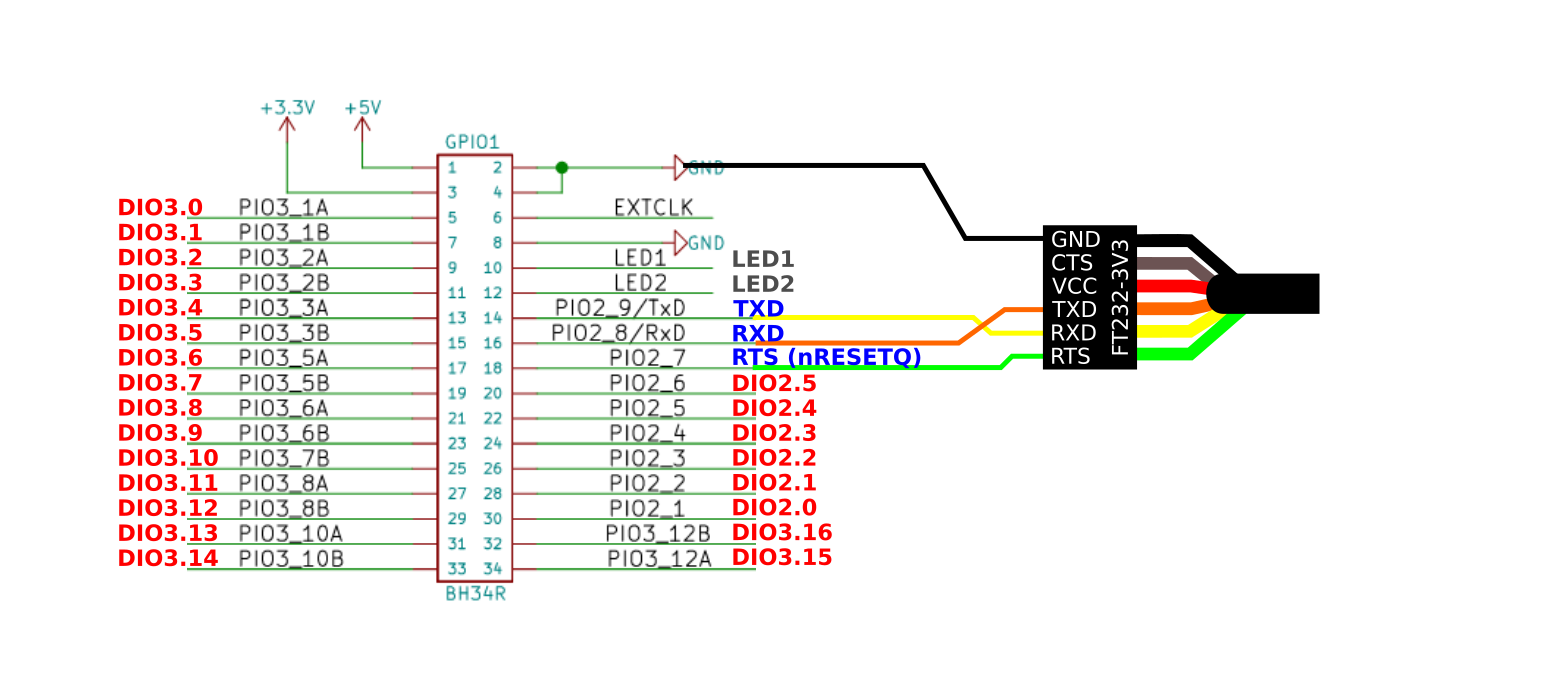
\includegraphics[width=1.4\textwidth]{olimex_io.png}
\end{center}

\newpage 

This J1a implementation for The Olimex ICE40 boards includes support for the following peripherals:
\begin{itemize}

\item 2x LEDs & 2x Button \index{Buttons}
\item GPIO connector \index{GPIO}
\item UART \index{UART}
\item SRAM (4 x 64k x 16bit accessable, 512kbyte total)\index{SRAM}
\item SPI flash (2 MByte) \index{SPI flash}

\end{itemize}

Access to peripherals is via the
\mach{io@} and \mach{io!} words.
Peripherals are port-mapped into a 16-bit IO address space.
Most ports are either read-only or write-only.
For read-only ports, writing to the port has no effect.
For write-only ports, reading from the port gives zero.

As an example of direct port access, this reads the buttons and sets the LEDS while also reporting the value to the serial console
\index{blink}

\begin{framed}
\begin{Verbatim}
\ output buttons to leds and terminal
: .bleds
begin
  $2000 io@
  3 rshift 3 xor
  dup .x
  $0004 io!
again
;
\end{Verbatim}
\end{framed}


\begin{framed}
\begin{Verbatim}
\ display button io state as hex 
: .buttons
begin
  $2000 io@ .x
again
;
\end{Verbatim}
\end{framed}


\begin{framed}
\begin{Verbatim}
\ Pulse each GPIO pin (D0=Fmax ... D15=Fmax/2^15)
: testio
$ffff 2 io!
begin
  65535 0 do
    i 1 io!
  loop
again
;
\end{Verbatim}
\end{framed}



\newpage
\section{Port Map}
\subsection{\$0001: GPIO data}

The read-write port at address \$0001 is for direct access to the GPIO1
connector. The port pins are assigned as follows (bottom row is closest to PCB):

\vspace{10pt}
\begin{tabular}{cccc}
\textbf{Connection} & \textbf{Top row pins} & \textbf{Bottom row pins} & \textbf{Connection} \\
\hline
5V  &  1 &   2 & GND \\
3V3 &  3 &   4 & GND \\
bit 0 &  5 &   6 & 100MHZ Clock \\
bit 1 &  7 &   8 & GND \\
bit 2 & 9  &  10 & LED1 \\
bit 3 & 11 & 12 & LED2 \\
bit 4 & 13 & 14 & TXD (out) \\
bit 5 & 15 & 16 & RXD (in) \\
bit 6 & 17 & 18 & RTS (in) \\
bit 7 & 19 & 20 & x \\
bit 8 & 21 & 22 & x \\
bit 9 & 23 & 24 & x \\
bit 10 & 25 & 26 & x \\
bit 11 & 27 & 28 & x \\
bit 12 & 29 & 30 & x \\
bit 13 & 31 & 32 & x \\
bit 14 & 33 & 34 & bit 15 \\

\end{tabular}
\vspace{10pt}

Correspondingly the port bits are assigned to pins as follows:

\vspace{10pt}
\noindent
\begin{bytefield}[endianness=big, bitwidth=2.0em]{16}
  \bitheader{0-15} \\
    \bitbox{1}{34} &
    \bitbox{1}{33} &
    \bitbox{1}{31} &
    \bitbox{1}{29} &
    \bitbox{1}{27} &
    \bitbox{1}{25} &
    \bitbox{1}{23} &
    \bitbox{1}{21} &
    \bitbox{1}{19} &
    \bitbox{1}{17} &
    \bitbox{1}{15} &
    \bitbox{1}{13} &
    \bitbox{1}{11} &
    \bitbox{1}{9} &
    \bitbox{1}{7} &
    \bitbox{1}{5}
\end{bytefield}
\vspace{10pt}

Note that pin direction is controlled by the corresponding bit the port at address \$0002.

\subsection{\$0002: GPIO direction}

Each of the 16 bits controls the direction of the corresponding pin of the GPIO connector.
0 sets the pin to input, 1 means sets the pin to output.
The bit-to-pin mapping is the same as for port \$0001.

\vspace{10pt}
\subsection{\$0004: LEDs}

The five on-board LEDS are controlled by write-only port at address \$0004.
Setting a bit to 1 lights the corresponding LED.

\vspace{10pt}
\noindent
\begin{bytefield}[endianness=big, bitwidth=2.0em]{16}
  \bitheader{0-15} \\
    \bitbox{14}{} &
    \bitbox{1}{\tiny{LED2}} &
    \bitbox{1}{\tiny{LED1}}
\end{bytefield}

Built-in word
\wordidx{leds}
writes to this port.

\subsection{\$0008: PIO output}

%  assign {PIO1_20, PIO1_18, PIOS_00, PIOS_02, PIOS_03} = PIOS;

Write-only port \$0008 controls the flash (SPI) outputs.

\vspace{10pt}
\noindent
\begin{bytefield}[endianness=big, bitwidth=2.0em]{16}
  \bitheader{0-15} \\
    \bitbox{13}{} &
    \bitbox{1}{\tiny{flash\\SCK}} &
    \bitbox{1}{\tiny{flash\\MOSI}} &
    \bitbox{1}{\tiny{flash\\CS}}
\end{bytefield}


\subsection{\$0010, \$0020, \$0040: SRAM}

The 16bit x 256k SRAM chip is connected to IO ports. These ports can be used to Read and Write up to 512kByte of data (in 4 banks of 128 kbyte)
The write port at address \$0010 is setting the 16 bit SRAM R/W address
The read-write port at address \$0020 is for writing and reading the 16 bit SRAM data
The write port at address \$0040 is controlling the SRAM data direction and R/W bits, and to set the upper 2 address bits. The words
\wordidx{sramw}, \wordidx{sramr} can be used to access these ports.

\vspace{10pt}
\$0010 SRAM Address register:

\vspace{10pt}
\noindent
\begin{bytefield}[endianness=big, bitwidth=2.0em]{16}
  \bitheader{0-15} \\
    \bitbox{16}{Address A15:A0}
\end{bytefield}

\vspace{10pt}
\$0020 SRAM Data register:

\vspace{10pt}
\noindent
\begin{bytefield}[endianness=big, bitwidth=2.0em]{16}
  \bitheader{0-15} \\
    \bitbox{16}{Data D15:D0}
\end{bytefield}

% { 11'b0, A17, A16, SRAM_nOE, SRAM_nWE, IO_DIR }
\vspace{10pt}
\$0040 SRAM Control register:

\vspace{10pt}
\noindent
\begin{bytefield}[endianness=big, bitwidth=2.0em]{16}
  \bitheader{0-15} \\
    \bitbox{11}{}
    \bitbox{1}{\tiny{A17}}
    \bitbox{1}{\tiny{A16}}
    \bitbox{1}{\tiny{nOE}}
    \bitbox{1}{\tiny{nWE}}
    \bitbox{1}{\tiny{DIR}}
\end{bytefield}




\subsection{\$0800: SB\_WARMBOOT control} \index{SB\_WARMBOOT} \index{reconfigure}

Write-only port \$0800 is an interface to the SB\_WARMBOOT module.
When activated, the FPGA loads a new configuration from external flash.
There can be up to four external configurations;
configuration 0 is the base SwapForth, and configurations 1-3 are available for other uses.
So to reload the base system:

\begin{Verbatim}
  4 $800 io!
\end{Verbatim}

\vspace{10pt}
\noindent
\begin{bytefield}[endianness=big, bitwidth=2.0em]{16}
  \bitheader{0-15} \\
    \bitbox{13}{} &
    \bitbox{1}{\tiny{BOOT}} &
    \bitbox{1}{\tiny{S1}} &
    \bitbox{1}{\tiny{S0}}
\end{bytefield}

\subsection{\$1000: UART data}

The read-write port at address \$1000 is for UART transmission or reception.
Writing to the port starts transmission of a byte, reading the port returns
the incoming byte.

Standard words
\wordidx{key}, \wordidx{key?} and \wordidx{emit}
can be used to access this port.

\vspace{10pt}
\noindent
\begin{bytefield}[endianness=big, bitwidth=2.0em]{16}
  \bitheader{0-15} \\
    \bitbox{8}{} &
    \bitbox{8}{byte}
\end{bytefield}

\subsection{\$2000: Buttons, SPI MISO and UART inputs}

Read-only port \$2000 contains the input signals from the
Buttons, SPI flash, and UART.

\vspace{10pt}
\noindent
\begin{bytefield}[endianness=big, bitwidth=2.0em]{16}
  \bitheader{0-15} \\
    \bitbox{11}{} &
    \bitbox{1}{\tiny{Button\\BUT2}} &
    \bitbox{1}{\tiny{Button\\BUT1}} &
    \bitbox{1}{\tiny{Flash\\MISO}} &
    \bitbox{1}{\tiny{UART\\key?}} &
    \bitbox{1}{\tiny{UART\\busy}}
\end{bytefield}

\clearpage
\addcontentsline{toc}{chapter}{Index}
\printindex

\end{document}
